\chapter{Application of Deep Learning in Segmenting Experimental Core-flooding Microtomography Images}
\section{Introduction}
The segmentation work flow described in Chapter 3 works well on the data in terms of quality, but it has some shortages. First, it has three main steps which are denoising, masking and segmentation, each step has few adjustable parameters, it is very time consuming to test the parameter combination for the best segmentation result in different imaging conditions. So the work flow is not a 'panacea' for all CT data. Second, it relies on the mask image segmented from reference scan, data that lack of such reference and suffer from poor contrast could not be accurately segmented using this work flow. Third, the overall processing time for one synchrotron experiment by the work flow is month-scale, which becomes a bottle-neck for the subsequent scientific analysis. So it is necessary to employ the state-of-art deep learning segmentation using convolutional neural networks (CNN) that can massively reduce the processing time meanwhile yield equally good segmentation.

\section{Deep learning for image segmentation}
Machine learning is a subset of artificial intelligence that can make self-modification through structured data to improve its output. One of the many applications of machine learning is computer vision, i.e. recognising objects from digital images. Image segmentation is one of the main tasks of computer vision. Various of machine learning algorithms have been powering image segmentation, for example from unsupervised K-means clustering \citep{lloyd1982least}, to supervised trainable Weka segmentation \citep{arganda2017trainable}. Deep learning is a more advanced subset of machine learning that use multiple layers of algorithms to create an 'artificial neural network'. With this layered structure of algorithms, machine can use each layer to hierarchically learn specific features of images, and produce better outcome with less human interference. The core of deep learning is the backpropagation algorithm \citet{lecun1989backpropagation} that allows discovery of intricate structure in large data set. Backpropagation uses these information to indicate the self-modification of its internal parameters (neurons) that are used to compute the representation in each layer from the previous layer. With large image data sets provided to deep neural network, machine can learn a computational model that represents the relation between raw image and segmentation, and this model can be used to predict the segmentation of data sets of similar kind.

\subsection{Convolutional Neural network}
CNNs \citet{lecun2015deep} are a class of deep neural network that have been proved effective in segmentation tasks (e.g. \citet{long2015fully}; \citet{krizhevsky2012imagenet}; \citet{girshick2014rich}). CNNs are specialised in processing data that has a grid-like topology, such as an image - digital images comprise arrays of pixels arranged in a grid and each pixel has a value for intensity. 

Convolutional neural network normally consists three kind of layers: convolutional layers, pooling layers and fully connected layers. For example \citet{krizhevsky2012imagenet} built the ground breaking CNN for image classification with five convolutional layers and three max pooling layers with a final fully connected layers. Fig.\ref{cnn} shows the generic architecture of CNN. 

\begin{figure}[htbp]
  \centering
  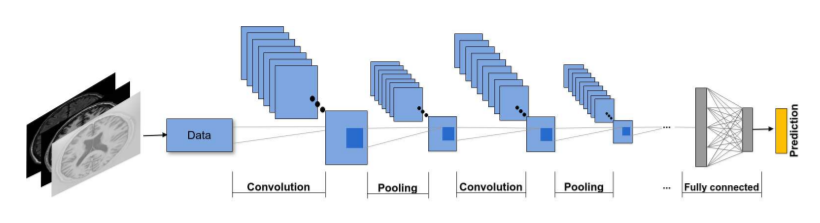
\includegraphics[width=1\textwidth]{\dir/figs/cnn.png}
  \caption{\citet{bernal2019deep}}
  \label{cnn}
\end{figure}

\subsubsection{Convolutional layer}
Convolution is essentially a mathematical operation on two functions $f(x),g(x)$ to produce the third function $h(x)$. $h(x)$ is the integral of the product of $f(x),g(x)$. In the context of CNN, convolutional layer uses a fixed sized matrix, i.e. a kernel, to operate convolution on a small local part of an image, then produce a feature map that extracting simple features such as edges, curves, corners and color patches (see for example Fig.\ref{featuremap}). The kernel will slide across the whole image and extract such simple features of the image. As the convolution process going, more complex and higher level features, such as eyes, hands are extracted in deeper convolutional layers.

\begin{figure}[htbp]
  \centering
  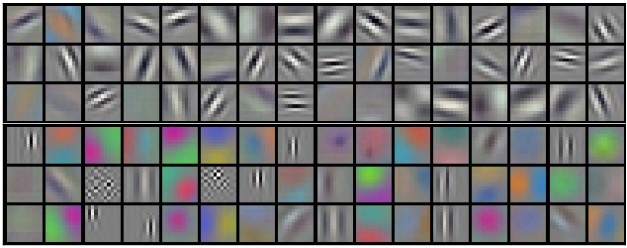
\includegraphics[width=1\textwidth]{\dir/figs/featuremap.png}
  \caption{Examples of feature map learned by \citet{krizhevsky2012imagenet}. The first convolutional layer is extracting local patterns such as edges and colour patches. The kernel size was $11\times11\times3$ and the image size was $224\times224\times3$. 3 is the channel depth and each represents one of the RGB colours for a coloured image.}
  \label{featuremap}
\end{figure}

\subsubsubsection{Non-linearity layer}
\label{nonlinearity}
Linear classifiers can only distinguish superficial patterns because they can only carve their input space into very simple regions \citep{lecun2015deep}. It may distinguish cats from dogs, but for more complex and sensitive tasks such as distinguish Samoyed dogs from wolves (both look alike but subtly different), non-linear classifiers are more suitable for the job. 
Non-linearity is achieved using a group of functions called activation functions after convolution, such as sigmoid function ($A=\frac{1}{1+e^{-x}}$), Tanh function ($tanh(x)=\frac{2}{1+e^{-2x}}-1$) and rectified linear unit (ReLU, $A(x) = max(0,x)$).

\paragraph{ReLU}
\begin{figure}[htbp]
  \centering
  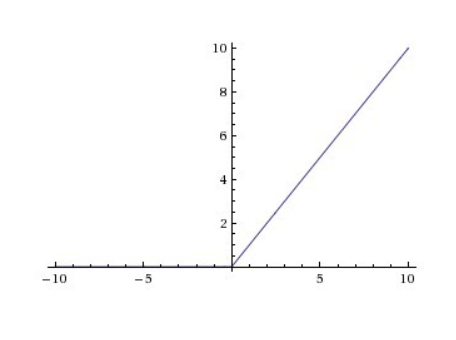
\includegraphics[width=1\textwidth]{\dir/figs/relu.png}
  \caption{relu}
  \label{relu}
\end{figure}

ReLU is one of the most commonly used activation function in CNN \citep{deng2014deep}, It gives an output x if x is positive and 0 otherwise (Fig.\ref{relu}). ReLU also slim down the network by making the activated neuron sparse and more efficient. Some variants of ReLUs such as LReLU, PReLU, RReLU \citep{xu2015empirical,he2015delving,maas2013rectifier} were also proposed to serve different learning scenarios.

\subsubsection{Pooling layer}
Following non-linear activation functions, the output is modified by a pooling (or subsampling) layer before proceeding to the next convolutional layer. Pooling serves mainly three purposes 1) to reduce the number of parameters, 2)alleviate over-fit and most importantly 3)increase translation invariant (i.e. preserving recognition of objects across variation in position, scale, illumination etc.) \citep{goodfellow2016deep}.

Among many pooling methods, max pooling is one of the most commonly used method. Max pooling is done by sub-sampling the maximum value of non-overlapping sub-regions of the image (see Fig.\ref{pooling} for example).

\begin{figure}[htbp]
  \centering
  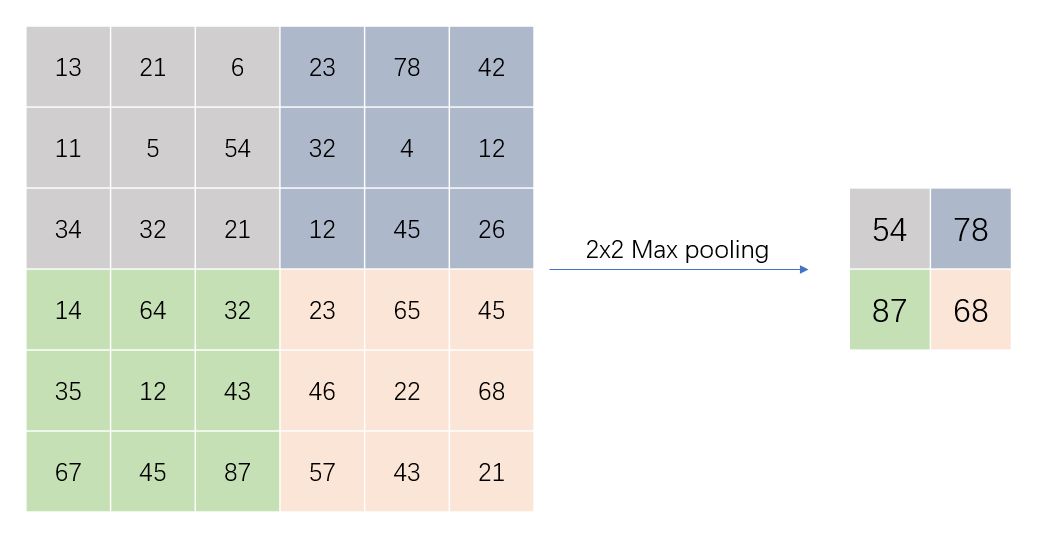
\includegraphics[width=1\textwidth]{\dir/figs/pooling.png}
  \caption{pooling}
  \label{pooling}
\end{figure}

\subsubsection{Fully connected layer}
Fully connected layer (FC layer) connects all units of the previous layers. It gives an overview to the complete output image. The output of this layer can be the prediction of class labels, or an intermediate layer for consecutive stacking of FC layers depending on the situation.

\subsection{CNN architecture: U-net}
\label{unet_architecture}
\citet{ronneberger2015u} proved the reliability of CNNs in segmenting neighbouring cells of biomedical images, which has similar difficulty with segmenting experimental multiphase flow images generated by microtomography. For this reason, among various of CNN architectures such as ResNet (\citet{he2016deep}), GoogLeNet (\citet{szegedy2015going}) and VGGNet (\citet{simonyan2014very}, we chose the CNN architecture 'U-Net' introduced by \citet{ronneberger2015u} as the CNN architecture used in this study.

\subsubsection{Network Architecture}
The U-net architecture is demonstrated in Fig.\ref{unet}. Built upon the neural network of \citet{ciresan2012deep}, U-net made improvement on the temporal efficiency, the use of context and the amount of data needed of \citet{ciresan2012deep}'s network.

\begin{figure}[htbp]
  \centering
  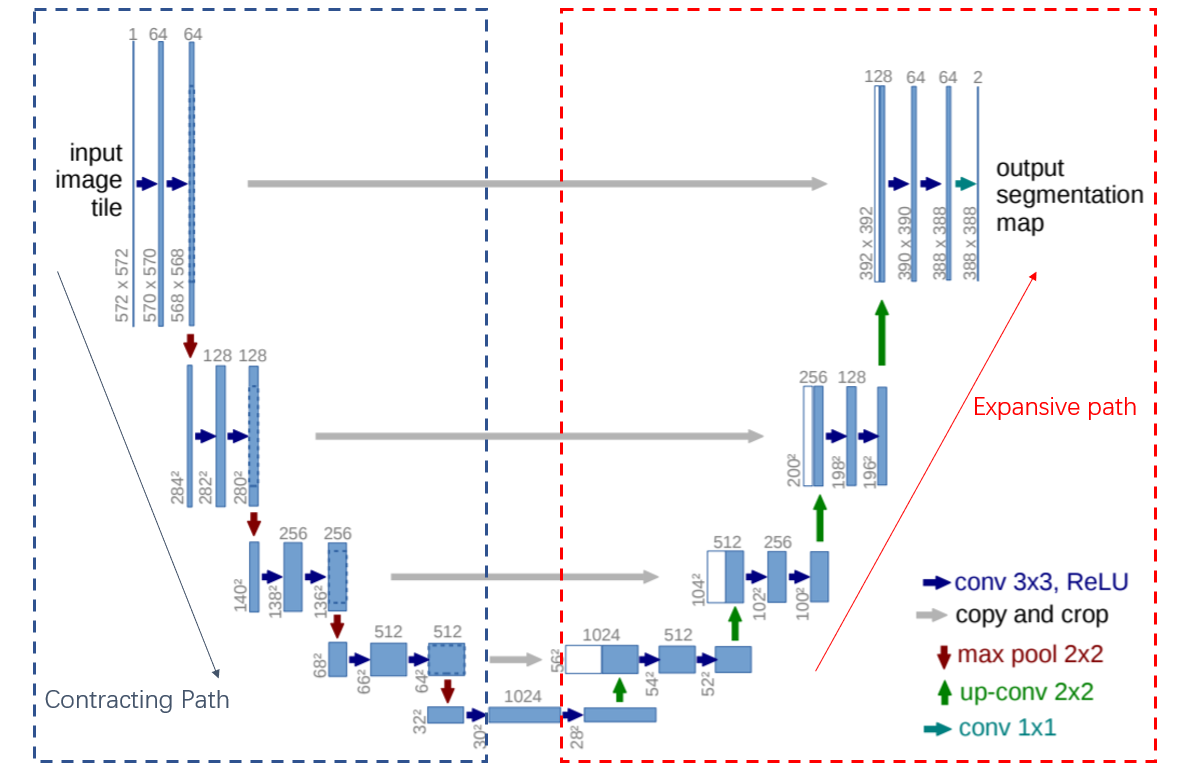
\includegraphics[width=1\textwidth]{\dir/figs/unet.png}
  \caption{modified from \citet{ronneberger2015u}}
  \label{unet}
\end{figure}

The network consists of contracting path (Fig.\ref{unet} left box) and expansive path (Fig.\ref{unet} right box). The contracting path, like conventional CNN, uses $3\times3$ convolution, followed by ReLU, then $2\times2$ max pooling for down-sampling. 

The expansive path up-samples the feature map with $2\times2$ up-convolution (the reverse operation of convolution), each up-convolution followed by $3\times3$ convolution with ReLU. A concatenation (joining) of feature map of the corresponding contracting path is applied to the up-convoluted feature map (Fig.\ref{unet} grey arrow copy and crop). The concatenation of cropped feature map from contracting path is necessary for compensating the lost border pixels during convolution. U-net does not have any FC layer, the final $1\times1$ convolution maps the total 64-component feature vectors to the desired number of classes. 

Comparing with \citet{ciresan2012deep}'s network, U-net has more feature channels in the up-sampling part, this allows the propagation of features to higher resolution layers. U-net also allows seamless segmentation of arbitrary size of input image. The original paper provided a Caffe \cite{jia2014caffe} implementation of U-net, in this study I used \citet{Jorispytorch}'s implementation of U-net in Pytorch environment. It has many tweakable options such as: 1) depth of the network, 2) number of filters per layer, 3) transposed convolutions vs. bilinear upsampling, 4) valid convolutions vs padding and 5) batch normalization.



\subsection{Principles of artificial neural network training}
Training an artificial neuron network segmentation model is a supervised learning process. The target of the neuron network model is to segment raw CT images as containing three phases: rock, oil and brine. First we collect a large data set of raw CT images, each image paired with its corresponding ground truth, i.e. the training data set. During training, the model is shown a raw image and produces an output of probability map that each pixel belongs to a specific category. We want the correct pixels have the highest probability than the wrong ones. At the onset of training, the prediction is random and unlikely to be correct everywhere. We use loss function (e.g. cross entropy loss for comparing probability distribution) to measure the error/distance between the output probability and the ground truth. By back-propagating the loss, the model attempts to adjust its internal parameters aiming at reducing the loss therefore make better prediction of the phases. The many internal adjustable parameters, namely neuron weights, are 'knobs' that define the input-output function of the model \citep{lecun2015deep}.

The neuron weights are adjusted using gradient vectors that computed by the machine. The gradient vectors indicate the error increments or decrements brought by tiny changes of neuron weights. A procedure called stochastic gradient descent (SGD) is commonly used to adjust the weights according to the gradient vectors. This is the internal mechanism for deciding how to turn the many 'knobs' of the model to minimise loss. The loss function, or objective function, is a higher-level, averaged representation of neuron weight values. Gradient vectors are indicators of the steepest descent of loss values. The loss values are step-wisely decreased to approach a minimum, where the prediction error is the lowest on average. 

One update of the neuron weights by one image is called a step, one full traverse of the training data set is called an epoch. The full training data set is usually iterated for tens to hundreds of epochs. During training, the loss is continuously reduced and eventually the decrement becomes infinitely small. Upon approaching the loss minimum, the model is well-trained and is then measured on a held-out set of examples, i.e. the test data set, to test the segmentation model's generalisation ability. Unlike the training data set that were 'seen' by the model for many iterations, the held-out testing data set is completely 'unseen' by the model. So the testing, like a mock test to a student, examines the model's prediction performance to unfamiliar real world data. 

\subsubsection{Accuracy evaluation}
The loss functions is more of a measurement of resemblance between input and output during training, it has limited indication of the final segmentation quality. Therefore more direct criteria of segmentation quality are needed to assess the model prediction. The resemblance between prediction and ground truth images is often quantified using intersection over union (IoU, e.g. \citep{rahman2016optimizing}), or receiver operating characteristic \citep{delong1988comparing} functions such as accuracy, precision, recall and F1 score etc. These criteria directly compare two binary images in a pixel-wise way, for example, precision measures the percentage of selected pixels that are correct, and recall measures the percentage of correct pixels that are selected, F1 score is the harmonic mean of precision and recall. These criteria directly indicate the quality of a segmentation. Trained models are tested with a testing data set using the above measurements. 

\subsubsection{Model generalisation and over-fit}
The ultimate goal of neural network training is predicting unfamiliar image segmentation, so a generalised model is crucial for this task. If the model is too specific to a homogeneous type of data, it is unable to make generalised prediction to new input. This problem is generally due to three reasons: 1)the model is trained with inadequate data, 2) the training data is biased, 3) the model is excessively trained with the same data. For inadequate training data, data augmentation strategy \citep{ronneberger2015u} can enlarge limited data set. For biased data set, make more heterogeneous data set can mitigate this problem. For the third situation, the exact amount of training needed for a model is crucial. With training data of suitable size and heterogeneity, if the amount of training is inadequate, the model is under-fit and can not make good prediction. If the amount of training is excessive, the model becomes over-fit and can not make general prediction to new data. Only the right amount of training can produce good model that can produce accurate segmentation to new data.

\begin{figure}[htbp]
  \centering
  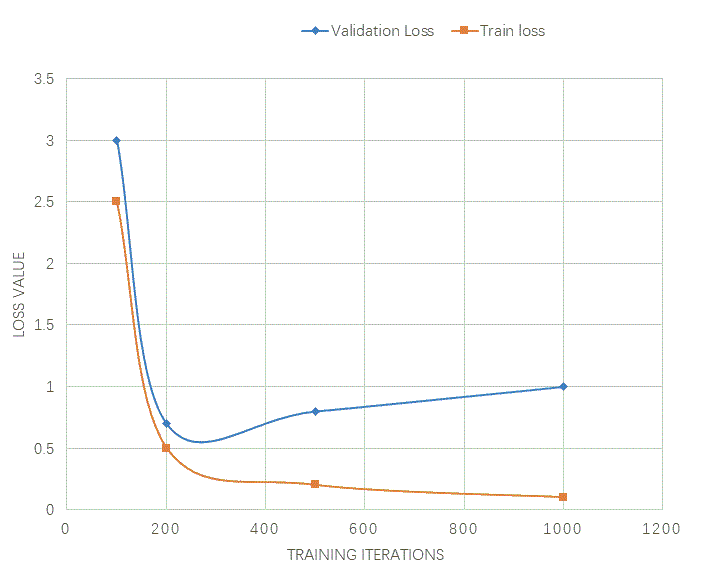
\includegraphics[width=1\textwidth]{\dir/figs/VALIDATION.png}
  \caption{}
  \label{validation}
\end{figure}

Validation is a syn-training process to keep track of the amount of training. Unlike training that updates the neuron weights every step and continuously makes improvement to the model, validation only checks the loss of the current model with a smaller data set, the validation data set. Fig.\ref{validation} shows a typical loss curve of training (orange) and validation (blue), the best training point is where the validation loss curve starting to increase (iteration=250), meaning that the model starts to over-fit from that point and prediction becomes less resemble to the ground truth. Stopping training at the validation loss turning point is called early-stopping and is regularly used to prevent over-fit.

\section{CNN training method for segmenting core-flooding experimental X-ray image}
\subsection{Software, functions and hyper-parameters in Training}
\subsubsection{Pytorch}
Pytorch \citep{paszke2017automatic} is an open-sourced deep learning ecosystem that provides tools and functions ready-to-use for deep learning projects. Comparing with other popular deep learning ecosystems such as Google's Tensorflow \citep{tensorflow2015-whitepaper} and UC Berkley's Caffe \citep{jia2014caffe}, Pytorch is more user-friendly, clear and simple in the process of neural network training. Pytorch is flexible and more suitable for small projects and prototyping. For the above reasons I used Pytorch to build the deep learning framework of this study.

\subsubsection{GPU acceleration}
Nvidia\texttrademark QuadroK5200 (8Gb) GPU allows CUDA \citep{cook2012cuda} to parallel computations on GPU and accelerate training. For same heavy computational load, CPU is efficient in complex computation of small amount, and GPU works better with simple computations of large amount, which is the convolution process in CNN training.

\subsubsection{CNN architecture}
U-net was the CNN architecture used in this study. Detailed description of U-net see \ref{unet_architecture}.

\subsubsection{Optimiser: Accelerating training}
Optimiser algorithms are used to accelerate training, there are a number of different built-in optimisers in Pytorch, such as Momentum \citep{sutskever2013importance}, RMSprop \citep{graves2013generating} and Adam \citep{kingma2014adam}. A simple test example of these three optimisers were run following \citet{MofanPython}'s online tutorial, and produced Fig.\ref{optimizer} to compare the performance of them.

\begin{figure}[htbp]
  \centering
  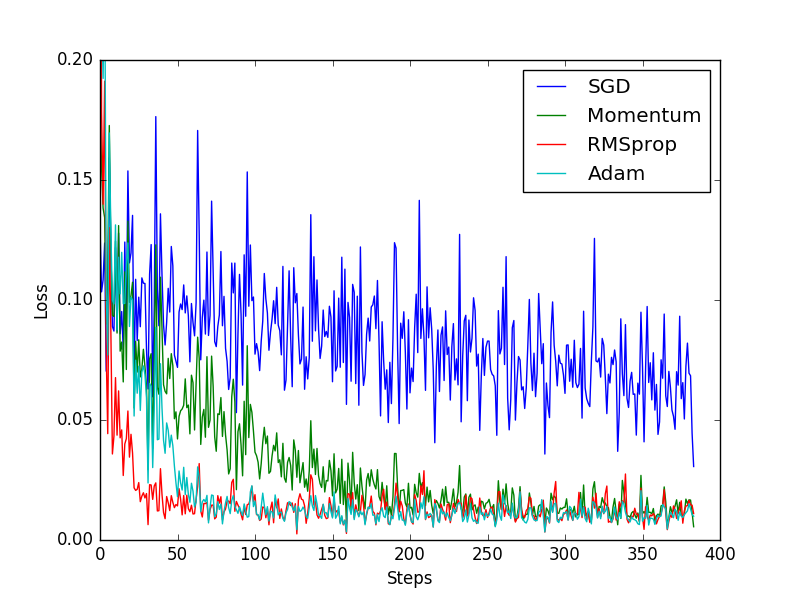
\includegraphics[width=1\textwidth]{\dir/figs/optimizer.png}
  \caption{}
  \label{optimizer}
\end{figure}

The advantage of using an optimiser is to reduce loss faster with less training. Fig.\ref{optimizer} shows RMSprop has the steepest loss reduction in this test and adam has similar effect of reducing loss, and Stochastic gradient descent (SGD, \citet{bottou2010large}), shows the loss reduction rate without an optimiser. I chose Adam as the optimiser to accelerate training because it is the most advanced optimiser among these four, in theory it combines momentum method and RMSprop method together.

\subsubsection{Activation function}
Activation function ReLU was used during training. See \ref{nonlinearity}.

\subsubsection{Loss function}
Pytorch built-in cross entropy loss was used as the loss function during training. It is one of the mostly used loss function for classification problems. Cross entropy loss describes the distance between two probability distributions, i.e. the euclidean distance of probability distribution produced by the network output and the ground truth in the context of this study.

At the first thought, one may wonder why not directly use classification error that measures the percentage of correctly predicted pixels? Because 51\% probability and 99\% probability that a pixel belongs to oil category both show the same result of true positive when use classification error, but the latter model that can make more certain prediction is much better than the former. Here the purpose of using loss function is to find a better model that making more reliable prediction, so we need to compare probability rather than classification.

To understand cross entropy loss, here we dig a bit into information theory. In information theory, the amount of information carried by an event can be quantified by it's probability of happening. For analogue, if one man received an email and he knows all the contents before receiving, the email carries zero information to the man. The man only get information when he knows less than 100\% of the email contents. When the man gets information that previously unknown, he will be 'surprised'. In the segmentation context, the degree of surprise brought by the model prediction 'surprisal' $s$, is calculated by:

\begin{equation}
S=log(\frac{1}{y_{i}})
\end{equation}

Where $y_{i}$ is the $i$th pixel of image $y$, containing information of probability that it belongs to a particular category, for example oil. Now take a weighted average of surprisals of all $n$ pixels of the model prediction, we get the entropy $e$ of this prediction:

\begin{equation}
e=\sum_{0}^{n}y_{i}log(\frac{1}{y_{i}})
\end{equation}

Generally, entropy refers to disorder or uncertainty, Claude Shannon \citep{shannon1948mathematical} used 'information entropy' to measure the amount of information conveyed by each event. In order to compare distance of two probability distributions $q_{i}$ and $p_{i}$, cross entropy $c$ is used:

\begin{equation}
c=\sum_{0}^{n}p_{i}log(\frac{1}{q_{i}})
\end{equation}

It measures the distance of the model prediction probability distribution $q_{i}$ and its ground truth $p_{i}$. Cross entropy $c$ decrease when $q_{i}$ and $p_{i}$ is more alike, and vice versa. By minimising the cross entropy loss, the model can make prediction that most resemble the ground truth. 

\subsubsection{Evaluation Functions}
\paragraph{Receiver operating characteristics }
ROC \citep{delong1988comparing} are measurements of classification errors. First we take probability above 95\% in model prediction as true, then calculate the true positive (TP), false positive (FP), true negative (TN) and false negative (FN) w.r.t. the ground truth. These four numbers can be used to calculate precision, recall, accuracy and F1 score, in this study we only use the Rand accuracy of each phase to evaluate segmentation quality:

\begin{equation}
    accuracy=\frac{TP+TN}{TP+TN+FP+FN}
\end{equation}

The reason for not using precision or recall is that they only take true positive into account but not true negative. The two phase may not necessarily present in every image. For those images that one fluid does not present, the true positive count of that fluid phase equals zero, thus the phase precision/recall is zero and could not represent the true accuracy. F1 is the harmonic mean of precision and recall thus also equals zero for the phase that does not present. In this study I only use accuracy for simplicity although exception can be coded to correct those wrong measurement by precision and recall.

\paragraph{Intersection over Union}
IoU is the ratio of the overlapping area of prediction and ground truth (intersection), with the total area that encompassed by prediction and ground truth (union):

\begin{equation}
    IoU=\frac{Area-of-Overlap}{Area-of-Union}
\end{equation}

A combination of these two metrics can define a good segmentation quality.

\subsubsection{Batch normalisation}
Firstly introduced by \citet{ioffe2015batch}, batch normalisation is a method to reduce internal covariate shift. Internal covariate shift is the change of input distribution to a learning system. Deep neural network amplifies even small changes of input whether relevant or irrelevant, leading to changes of the internal layers of the neural network. Batch normalisation is added before each non-linearity layer to achieve better training outcome.

\subsubsection{Hyper-parameters}
Hyper-parameters are readily defined parameters that control the overall learning process. Such as epochs, batch size, learning rate and regularisation.

\paragraph{Epochs} defines the total training epochs, i.e. the number of iterations to traverse the full training set.

\paragraph{batch size} defines the number of training images that being sent to the network at one step, called a mini-batch.

\paragraph{Learning rate} defines the speed of learning. An appropriate learning rate can make training loss converge within a reasonable training time, and meanwhile prevent divergent of the loss function.

\begin{figure}[htbp]
  \centering
  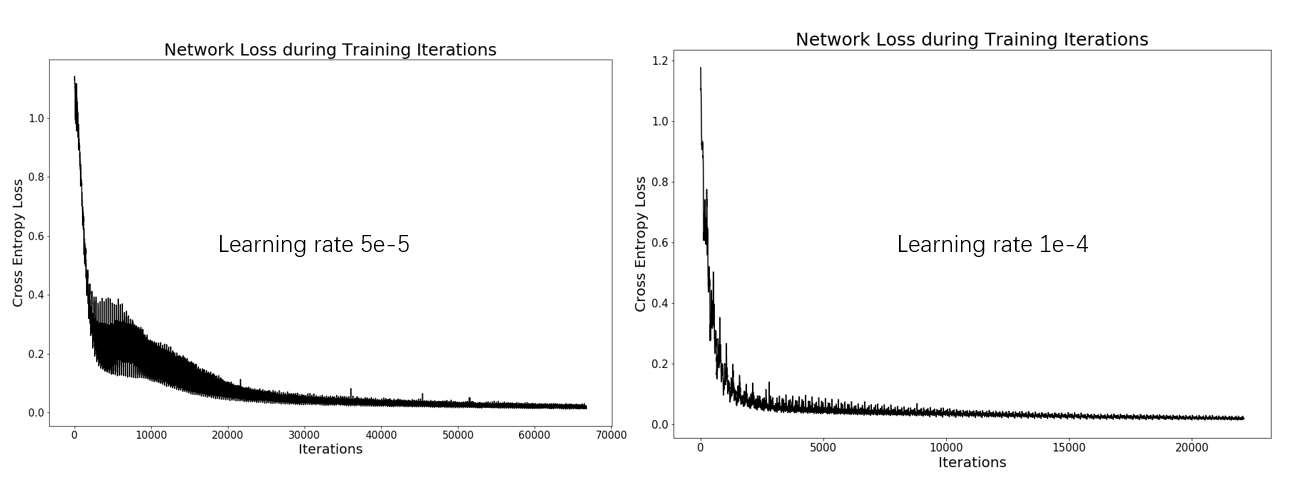
\includegraphics[width=1\textwidth]{\dir/figs/learninrate.png}
  \caption{}
  \label{learninrate}
\end{figure}

A test example of different learning rate shows in Fig.\ref{learninrate}, learning rate $5^{-5}$ is too low and lead to slower convergence of the loss curve (65000+). Learning rate $1^{-4}$ is appropriate that the loss curve does not diverge and converge faster (20000+) and smoother. For even higher learning rate, the loss will oscillate and hard to converge.

\paragraph{Regularisation} is a method to alleviate over-fitting by penalising high-valued regression coefficients, i.e. it reduces redundant parameters and slim down the model. In this study I used L2 regularisation (or Ridge Regularisation) that penalise the sum of squared weights. There is also L1 regularisation that penalise the sum of absolute values of weights. (The mathematical details of L1 and L2 regularisation is beyond the scope of the context)

\subsection{Data preparation}
A total of 18 CT volumes were used to train the CNN model. Each CT volume consists of raw images of size $1004 \times 1646 \times 1646$ and each paired with the corresponding ground truth images. The 18 CT volumes were split into 14:2:2 for training, validation and testing. A total of 14k+ images were used to train the CNN.

\subsubsection{Ground-truthing}
The ground truth images were segmented by seeded random walker described in chapter 3. 

The deep learning approach applied herein to analyse microtomography data differs from typical CNN application of segmenting objects like, e.g., a cat or a person. In such conventional approaches, training data sets are collections of thousands of manually segmented images. However, manual, genuine ground-truthing for all training data is unfeasible because of the highly irregular, complex, multi-scale or even fractal nature of pore-scale images. 

Thus high-quality microtomographic scans obtained before the initiation of the experiment are segmented using the random walker algorithm and used for training, along with high quality scans of the pore space with two fluids present. The ground truth segmentation images, although are not genuine ground truth, are the best possible segmentation that can be considered as the closest ground truth (Fig.\ref{test_original}). 

\begin{figure}[htbp]
  \centering
  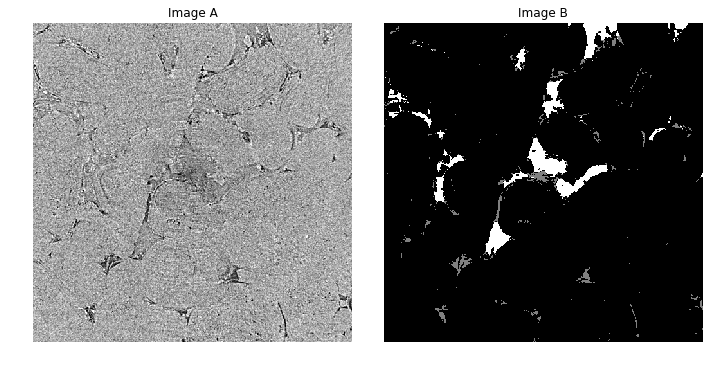
\includegraphics[width=1\textwidth]{\dir/figs/17_test_original.png}
  \caption{}
  \label{test_original}
\end{figure}

\subsubsection{Resizing of raw images}
The images, when loaded into the network, were down-sampled and cropped to $496\times496$. This size is reasonable for our GPU capibility (Nvidia\texttrademark Quadro K5200 8Gb) and the input image size is the multiple of $2^{depth-1}$
which satisfies the sampling process. 

\subsubsection{Intensity normalisation}
The pixel values were normalised to 0-1 using below equation to minimise intensity shift across images.

\begin{equation}
I[i]_{Nj}=\frac{j-I[i]_{min}}{I[i]_{max}-I[i]_{min}}
\end{equation}

where the normalised pixel $Nj$ of image $I[i]$ is calculated by: the difference of the original value of pixel $j$ with the minimum value $I[i]_{min}$ in image $I[i]$, divided by the difference of the maximum value with the minimum value $I[i]_{min}$ in image $I[i]$. It alleviated the intensity shift across images such as image A is overall brighter than image B.

\subsection{Training}
Prior to training, essential python packages for CNN training such as Pytorch \citep{paszke2017automatic}, Numpy \citep{van2011numpy} were imported into Python 3 environment. U-net CNN architecture implemented by \citet{Jorispytorch} was imported as the initial CNN model. 

\begin{figure}[htbp]
  \centering
  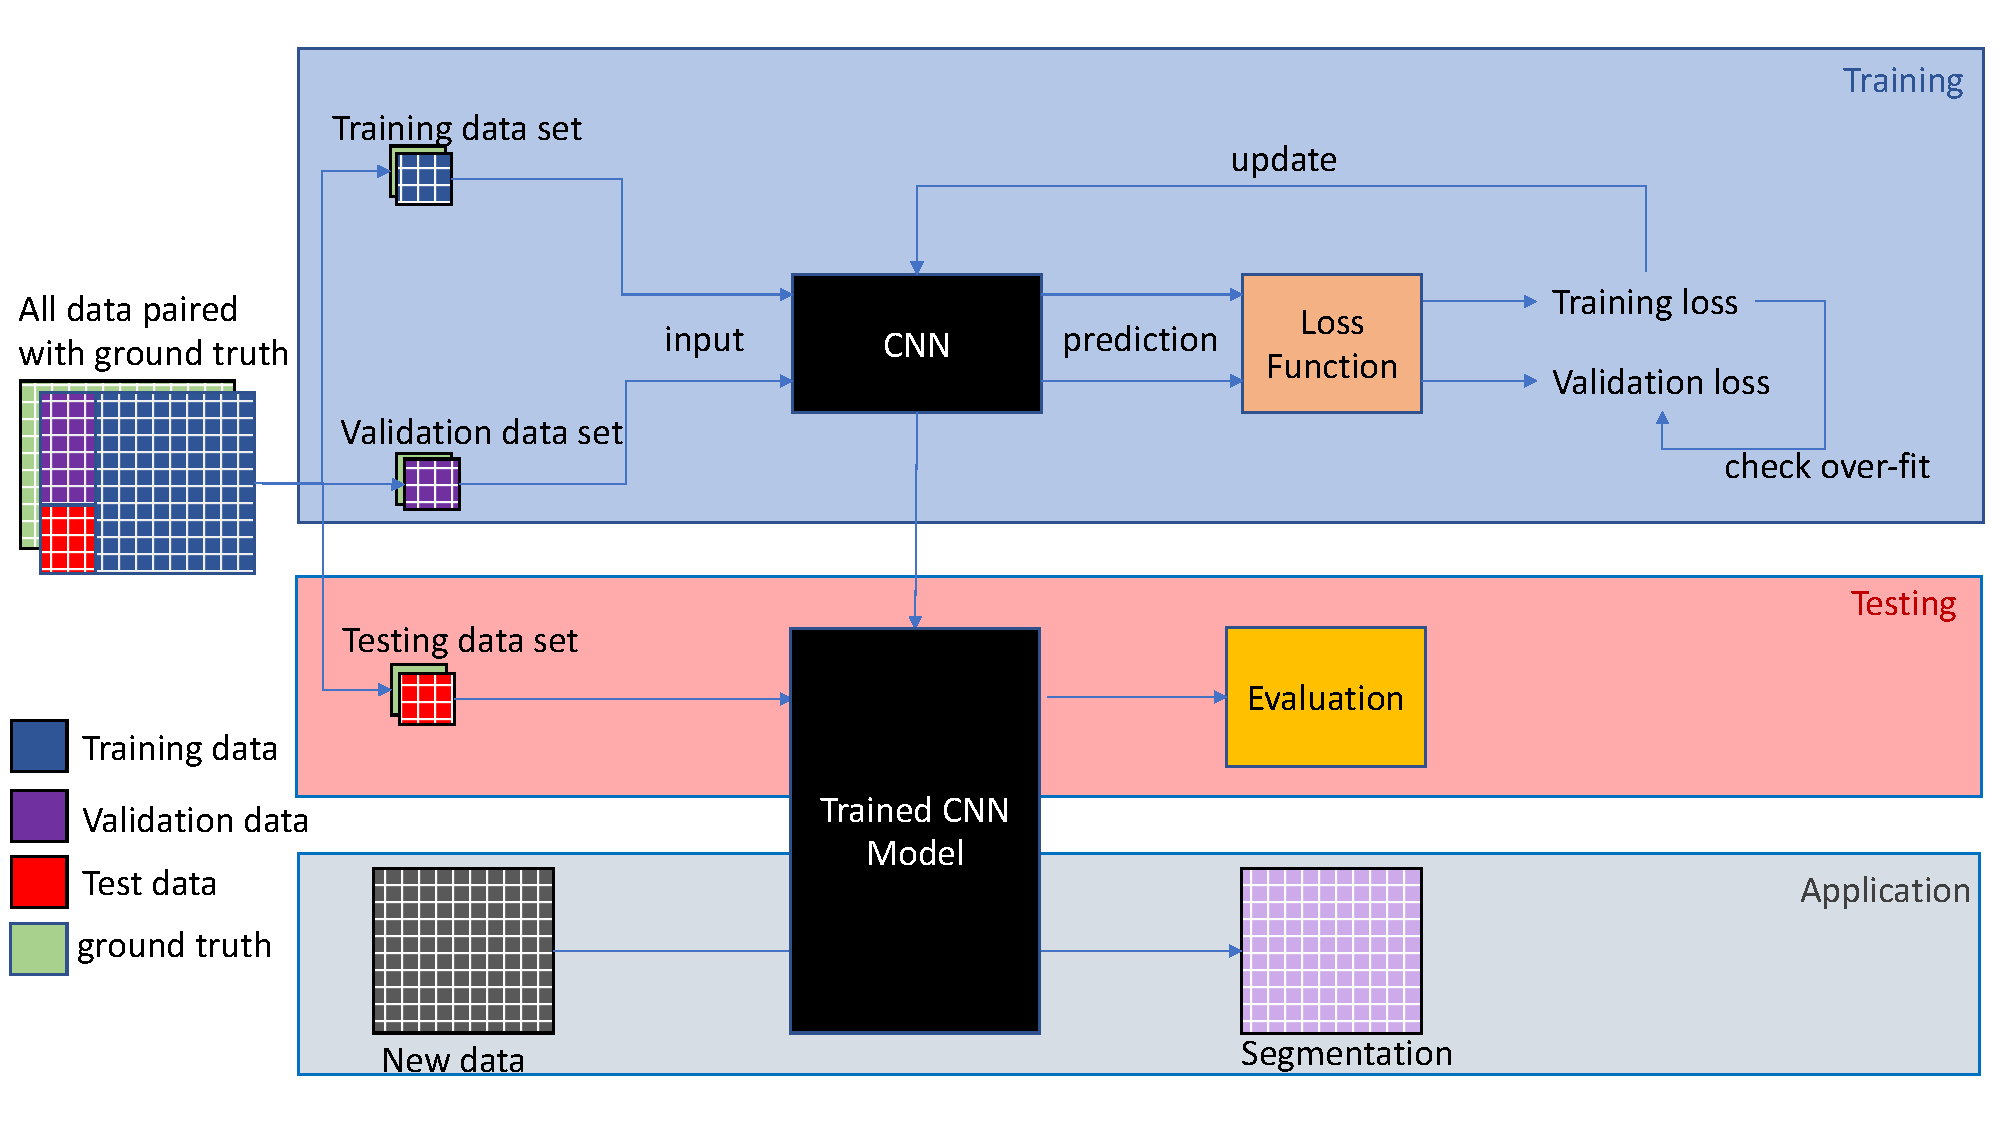
\includegraphics[width=1\textwidth]{\dir/figs/workfl.pdf}
  \caption{}
  \label{workfl}
\end{figure}

For one epoch, during each training step a raw image from the training data set was input into the CNN model, and a prediction of the three phase segmentation (oil, water, solid) was then produced by the CNN model. The segmentation was compared with the corresponding ground truth images by the cross entropy loss and yield a training loss value. The training loss was back-propagated to the network and the neuron weights were updated accordingly trying to minimise the loss. The loss gradually decreased as the training went on. The epoch ended when all images in the training set were traversed.

\subsection{Validation}
After each epoch, validation process measured the validation loss of the current model to prevent over-fit. A traverse of the validation data set by the model calculated the current validation loss, but there was no back-propagation of the loss so the model stayed unchanged. The training would proceed to the next training epoch if the validation loss was not increasing. The new epoch would repeat traversing the training data set but with a shuffled input sequence so the way that neuron weights being updated is different.

The best fit model was found at the epoch when the validation loss started increasing, because after this epoch the model started over-fit.

\subsection{Testing}
The trained model was tested using the held-out test data set. Accuracy and IoU was measured from the model prediction to assess the quality of segmentation of unfamiliar data.

\section{Results}
\subsection{Training result}
The CNN model was trained for 34 epochs using the above described methods. Fig.\ref{training_result} shows the loss values and accuracy and IoU measurements evolving through the training process. The total training time was 205.4 hours. 

The upper image shows the validation accuracy of the three phases: oil, brine, and rock (background). And three-phase IoU was also calculated. All measurements have reached above 98\%, and after the 28th epoch the accuracy stopped increasing.

The lower image shows the training loss versus validation loss. Training loss decreased monotonically from 1.1 to 0.02 during training. The validation loss crossed over the training loss at the 18th epoch, after some epochs of further subtle fluctuation, validation started increasing, although of a tiny amount, at the and this figure indicates the over-fit point at the 28th epoch. It is very difficult to identify the validation error increase on the figure because the increment is subtle, the criterion of early stopping was set as validation error increasing for consecutive five epochs. It is sure that the validation error will increase if training continues, I stopped training here because the best-fitting point at the 28th epoch has already been found. The overall decrement of the validation loss was tiny, it is difficult to see the very obvious u-shaped turning point paradigm because the curvature will take unrealistic time to form.

\begin{figure}[htbp]
  \centering
  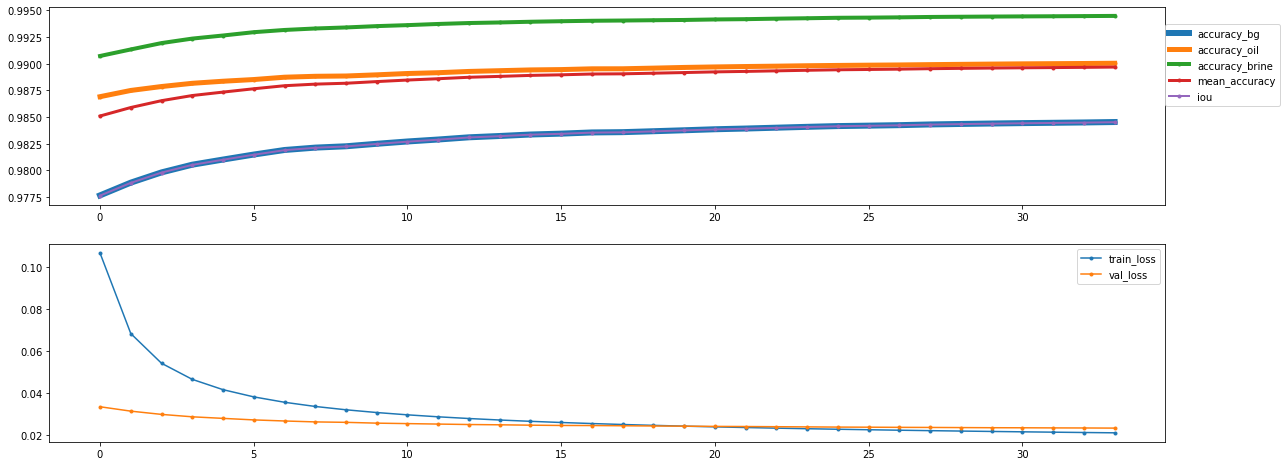
\includegraphics[width=1\textwidth]{\dir/figs/training_result_23oct}
  \caption{}
  \label{training_result}
\end{figure}

Noticing that the validation loss only changed for a very small amount, and it was already low from the first training epoch. This is because the training data set is considerably large, and the patterns are relatively simple and mostly dependent on its grey value, the model can learn a lot at the first epoch of training. The rest of the training was fine-tuning of the parameters for the very scarce but problematic features.

Another observation worth for attention is that the validation loss is relatively stable, while the training loss kept decreasing. This can be explained by the fact that the training data set is a time series that the adjacent ones are very similar, the validation set is also very similar to the training set which has the adjacent time stamp to it, thus the network learned well. However the validation set is very different from the early time stamps, so the later part of the training was spent on learning these trans-timestamp differences.

In the accuracy plot, the IoU curve (purple) is almost overlapping with the solid (blue), this is a coincidence due to the nature of these two evaluation functions. Accuracy measures the percentage of correct pixels among all pixels of one phase, and IoU measures the ratio of overlapping area among all area of the total three phases. The rock here has the largest constituent of the three phases, and therefore caused this overlap. The three phase accuracy, mean accuracy and the IoU all stopped increasing at the 28th epoch, this is consistent with the validation loss curve turning point at the 28th epoch.

Fig.\ref{11-29} shows the CNN model segmentation improvement during training epochs. The raw CT image was from the test data set so it guarantees that the input image is new to the model. The first row shows the raw CT image which is very noisy, and the CNN segmentation result at the 11th epoch of training, and the corresponding ground truth image. The second row shows the CNN segmentation result at the best-fit epoch which is the 29th epoch. The comparison of two segmentation shows that at the 11th epoch, the rock boundary is blurry, only part of the brine phase (yellow) is segmented with poor boundary sharpness, and many are confused with the rock. Large part of the oil phase (magenta) have blurry boundary and has lots of mis-classification. The second raw shows the segmentation result of the same CT image by the best-fit model which at the 29th epoch, and the same corresponding ground truth. The segmentation result is very resemble to the ground truth, and the phase boundary is sharp. So we can conclude that the CNN segmentation model has been successfully trained and waiting to be fully tested and challenged with new data.

\begin{figure}[htbp]
  \centering
  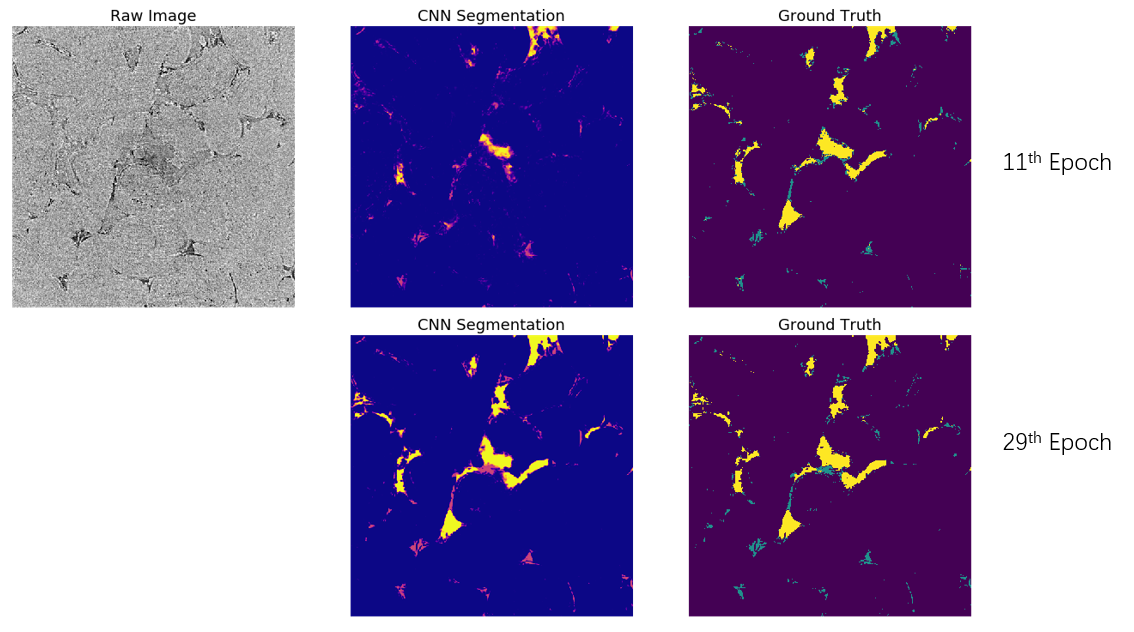
\includegraphics[width=1\textwidth]{\dir/figs/11-29}
  \caption{}
  \label{11-29}
\end{figure}

\subsection{Probability assessment}
The CNN does not directly output segmentation image, but a grid-like data (called Tensor in Pytorch environment) that indicating 'scores' of segmentation categories. These scores can not be directly used to segment objects because some components could be negative, or greater than one, or not sum to one. By applying a Softmax function, the scores will be rescaled to 0-1, and sum to one. Thus the Softmax function rescales the CNN output into a probability map that all components are in the interval $(0,1)$ and $oil+brine+solid=1$, meaning the categorical distribution of the three phases. I take the probability > 95\% as true, the rest as false, and convert the CNN output into the final segmentation. The probability map can be also used to assess the segmentation reliability (Fig.\ref{probmap}).

\begin{figure}[htbp]
  \centering
  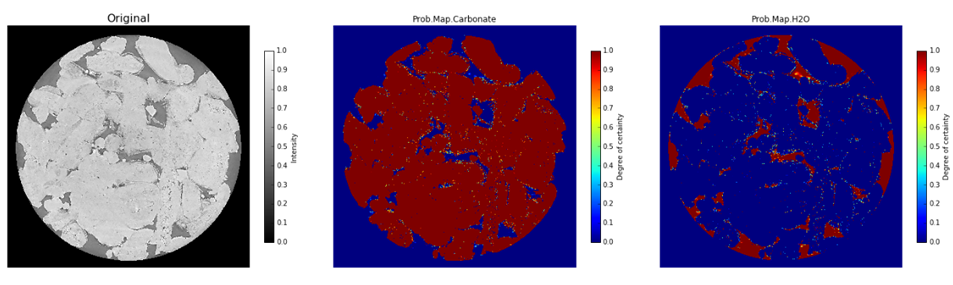
\includegraphics[width=1\textwidth]{\dir/figs/probmap}
  \caption{}
  \label{probmap}
\end{figure}

Fig.\ref{probmap} first row shows a raw CT image and its corresponding ground truth image. The second row shows the probability maps that converted from the direct CNN output by the Softmax function. The probability map is sized (3, width, lenght), where 3 means a stack of three maps of each particular phase, Fig.\ref{probmap} shows the three phase probability maps of solid, oil and brine. The probability distribution (0,1) is mapped with a blue-white-red colour map, where 0 means zero likely-hood that a pixel belongs to the particular phase, and 1 means 100\% likely-hood. Any probability value in-between 0-1 has some degree of uncertainty, the more it deviates from 0 or 1, the more uncertain the prediction is. 0.5 is the most uncertain case, meaning that the machine has no preference of this pixel's belonging. The likely-hood of solid, oil and brine sums up to one.

By visually checking the portion of whitish colours on the probability map, we can make intuitive assessment of the prediction reliability. The probability maps showing in Fig.\ref{probmap} has very few uncertain pixels, mainly located at rock boundaries and fluid interface. The probability map is also consistent with the accuracy evaluation in Fig.\ref{training_result}, the accuracy of the three phase from high to low is brine, oil then rock. On the probability map we also see fewest uncertainty on the brine map and then oil, and rock has the most uncertain pixels among the three. We can conclude the CNN provided a very reliable segmentation result. Quantitative assessment can be also made by further investigating of the probability maps.

\subsection{Testing}
The test result of the final CNN model shows the mean three-phase accuracy of 99.01\%, and phase accuracy of rock 98.51\%, brine 99.34\% and oil 99.16\%. IoU is 98.51\%. 

One example segmentation image, and the three-phase probability maps by testing is shown in Fig.\ref{testsegprob}. The test result shows very high quality segmentation, which is very close to its ground truth, and the probability map shows very certain phase probabilities that only very few pixels are ambiguous. However at some brine clusters, there is a thin layer of segmented oil between brine and rock, which does not occur in the ground truth segmentation. This is also expressed in the probability maps - many uncertainties are located at the phase boundaries, showing high difficulty of segmenting the phase boundaries. This difficulty of segmenting phase boundaries is due to the partial volume effect that affects the sharpness of the boundary. The wettability of this rock sample allows oil as the wetting phase to form oil film above the rock surface, but the rock surface roughness and the resolution of the CT may not allow the oil films to be identified on the CT image, so this 'oil film' present in the segmentation is reckon as misclassification.

\begin{figure}[htbp]
  \centering
  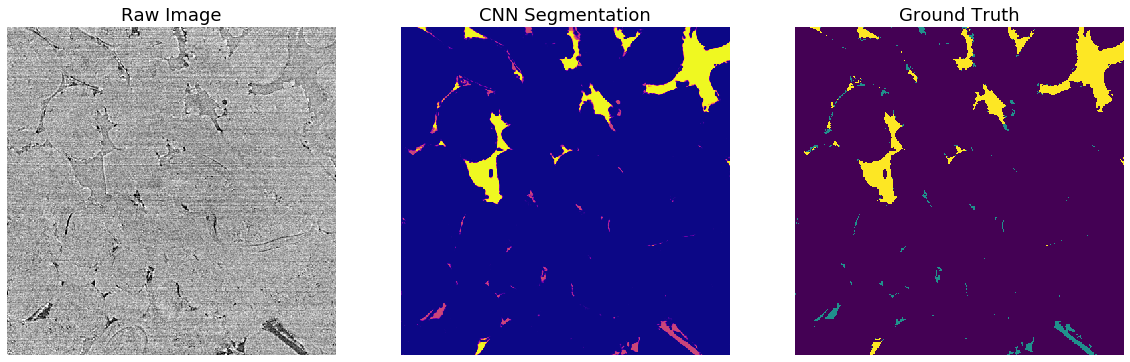
\includegraphics[width=1\textwidth]{\dir/figs/testseg}
  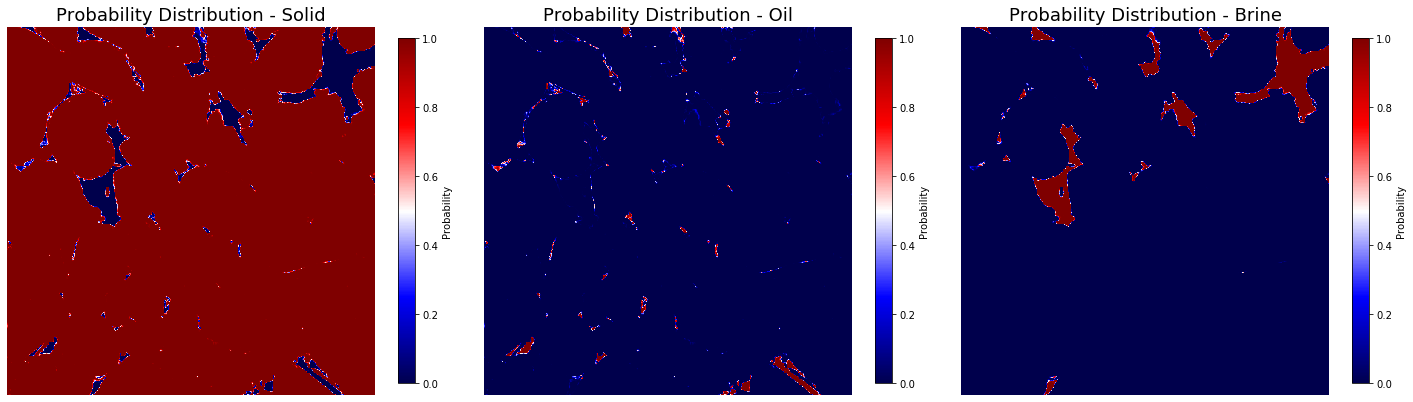
\includegraphics[width=1\textwidth]{\dir/figs/testprob}
  \caption{}
  \label{testsegprob}
\end{figure}

External standards of the conservation of the pore space is also used to evaluate the segmentation reliability. The experimental procedures guarantee that the pore space is saturated with only brine and oil. The proportion of oil and brine in the pore space is changing through the experiment, but the sum oil and brine volumes should always equal to the pore space. Fig.\ref{accumulative} shows the accumulative phase pixels of the CNN segmentation of a test CT volume. In this testing CT volume segmentation, the three phase - rock, oil and brine, has very close total volume with the ground truth. The sum of brine and oil pixels is 6,653,234 pixels. The ground truth sum, which equals to the pore space, is 6,975,417 pixels. The difference is 4.6\% which can be reckon as the segmentation error. The difference of segmentation with ground truth for brine, oil and rock phase are +4.2\%, +5.3\% and less than -0.1\% respectively. 

\begin{figure}[htbp]
  \centering
  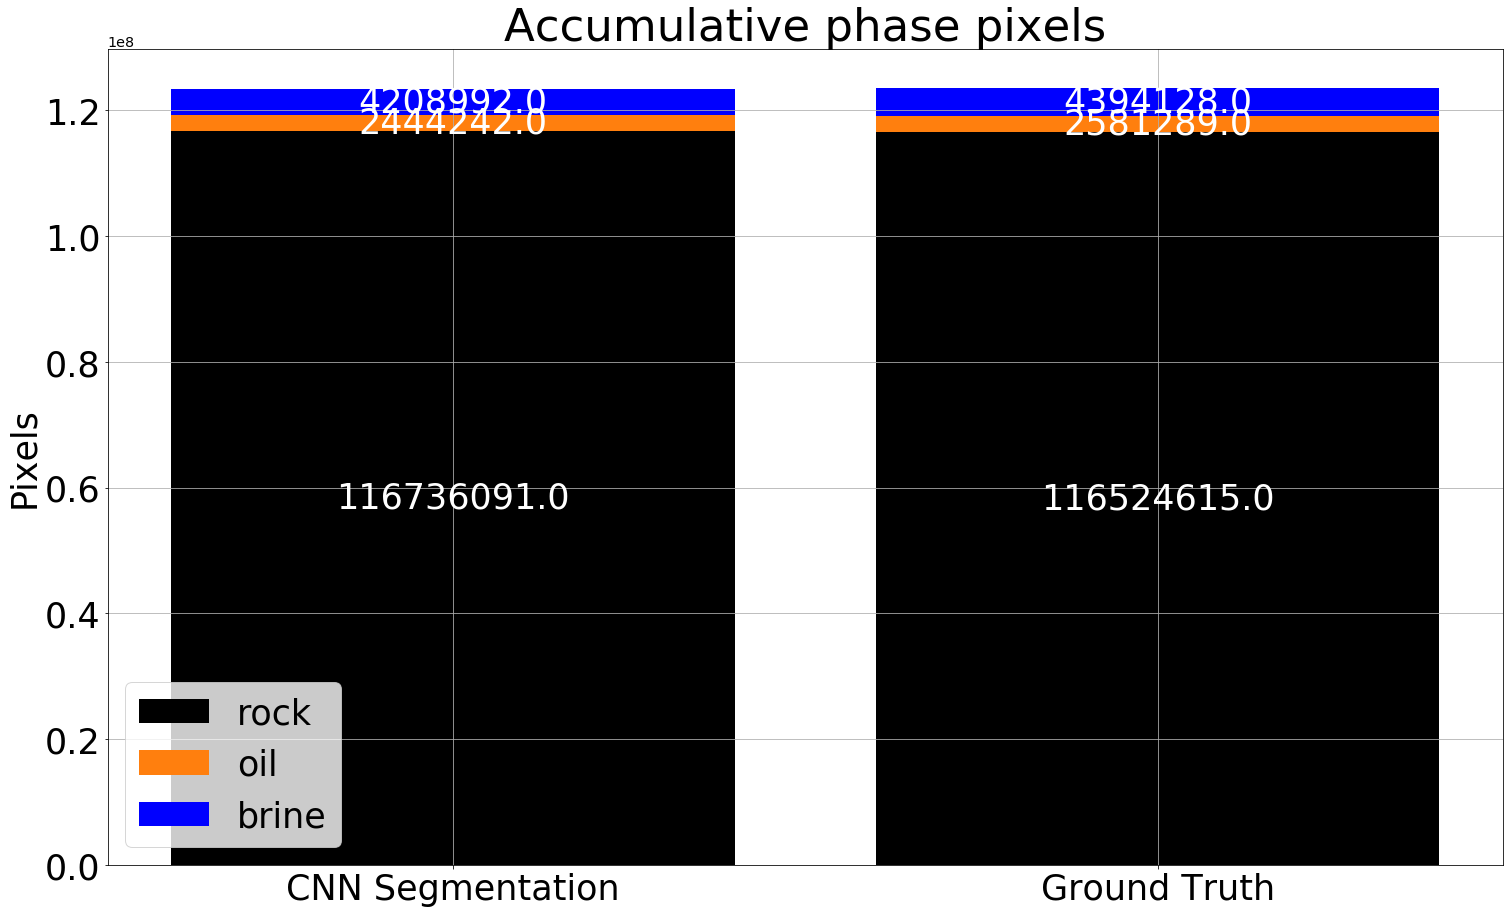
\includegraphics[width=1\textwidth]{\dir/figs/accumulative}
  \caption{}
  \label{accumulative}
\end{figure}

In summary, the CNN segmentation tends to misclassify a minor amount of rock as either one of the fluids, which often on the rock boundary. And some pixels in the rock-brine interface tends to be misclassified as brine due to the partial volume effect. Overall the CNN segmentation has very high accuracy and reliability. 

\section{Discussion}
\subsection{Segmentation robustness}
The CNN model robustness was examined with three types of artificial image degradation: blurring, noising and ring artefact, which are all common in CT image processing (Fig.\ref{noisetest}). The degradation effects were all applied on the same image from the testing data set.

The increasing degree of blurring was added to the image by convolving the image with a Gaussian function, by increasing the \textsigma that representing the standard deviation of the normal distribution (as known as Gaussian distribution). This mimics the blurring due to excessive filtering during the CT reconstruction often with TomoPy (Fig.\ref{noisetest} first row).

The second type of degradation is noising the image by Gaussian noise. Gaussian noise is a statistical noise with the probability density function of Gaussian distribution. Similarly, by increasing the \textsigma that representing the standard deviation of the Gaussian distribution, the image is increasingly noised. This mimics the common noise during CT image acquisition (Fig.\ref{noisetest}). 

The third type of degradation is ring artefact. Ring artefact is a common CT artefact that usually due to miscalibration or failure of the detector element (See Chapter2.). Ring artefact was added to the image by generating concentric circles with different radii and intensities at a fixed coordinate. To make more severe ring artefact I increase the number of iterations of generating circles (Fig.\ref{noisetest}).

\begin{figure}[htbp]
  \centering
  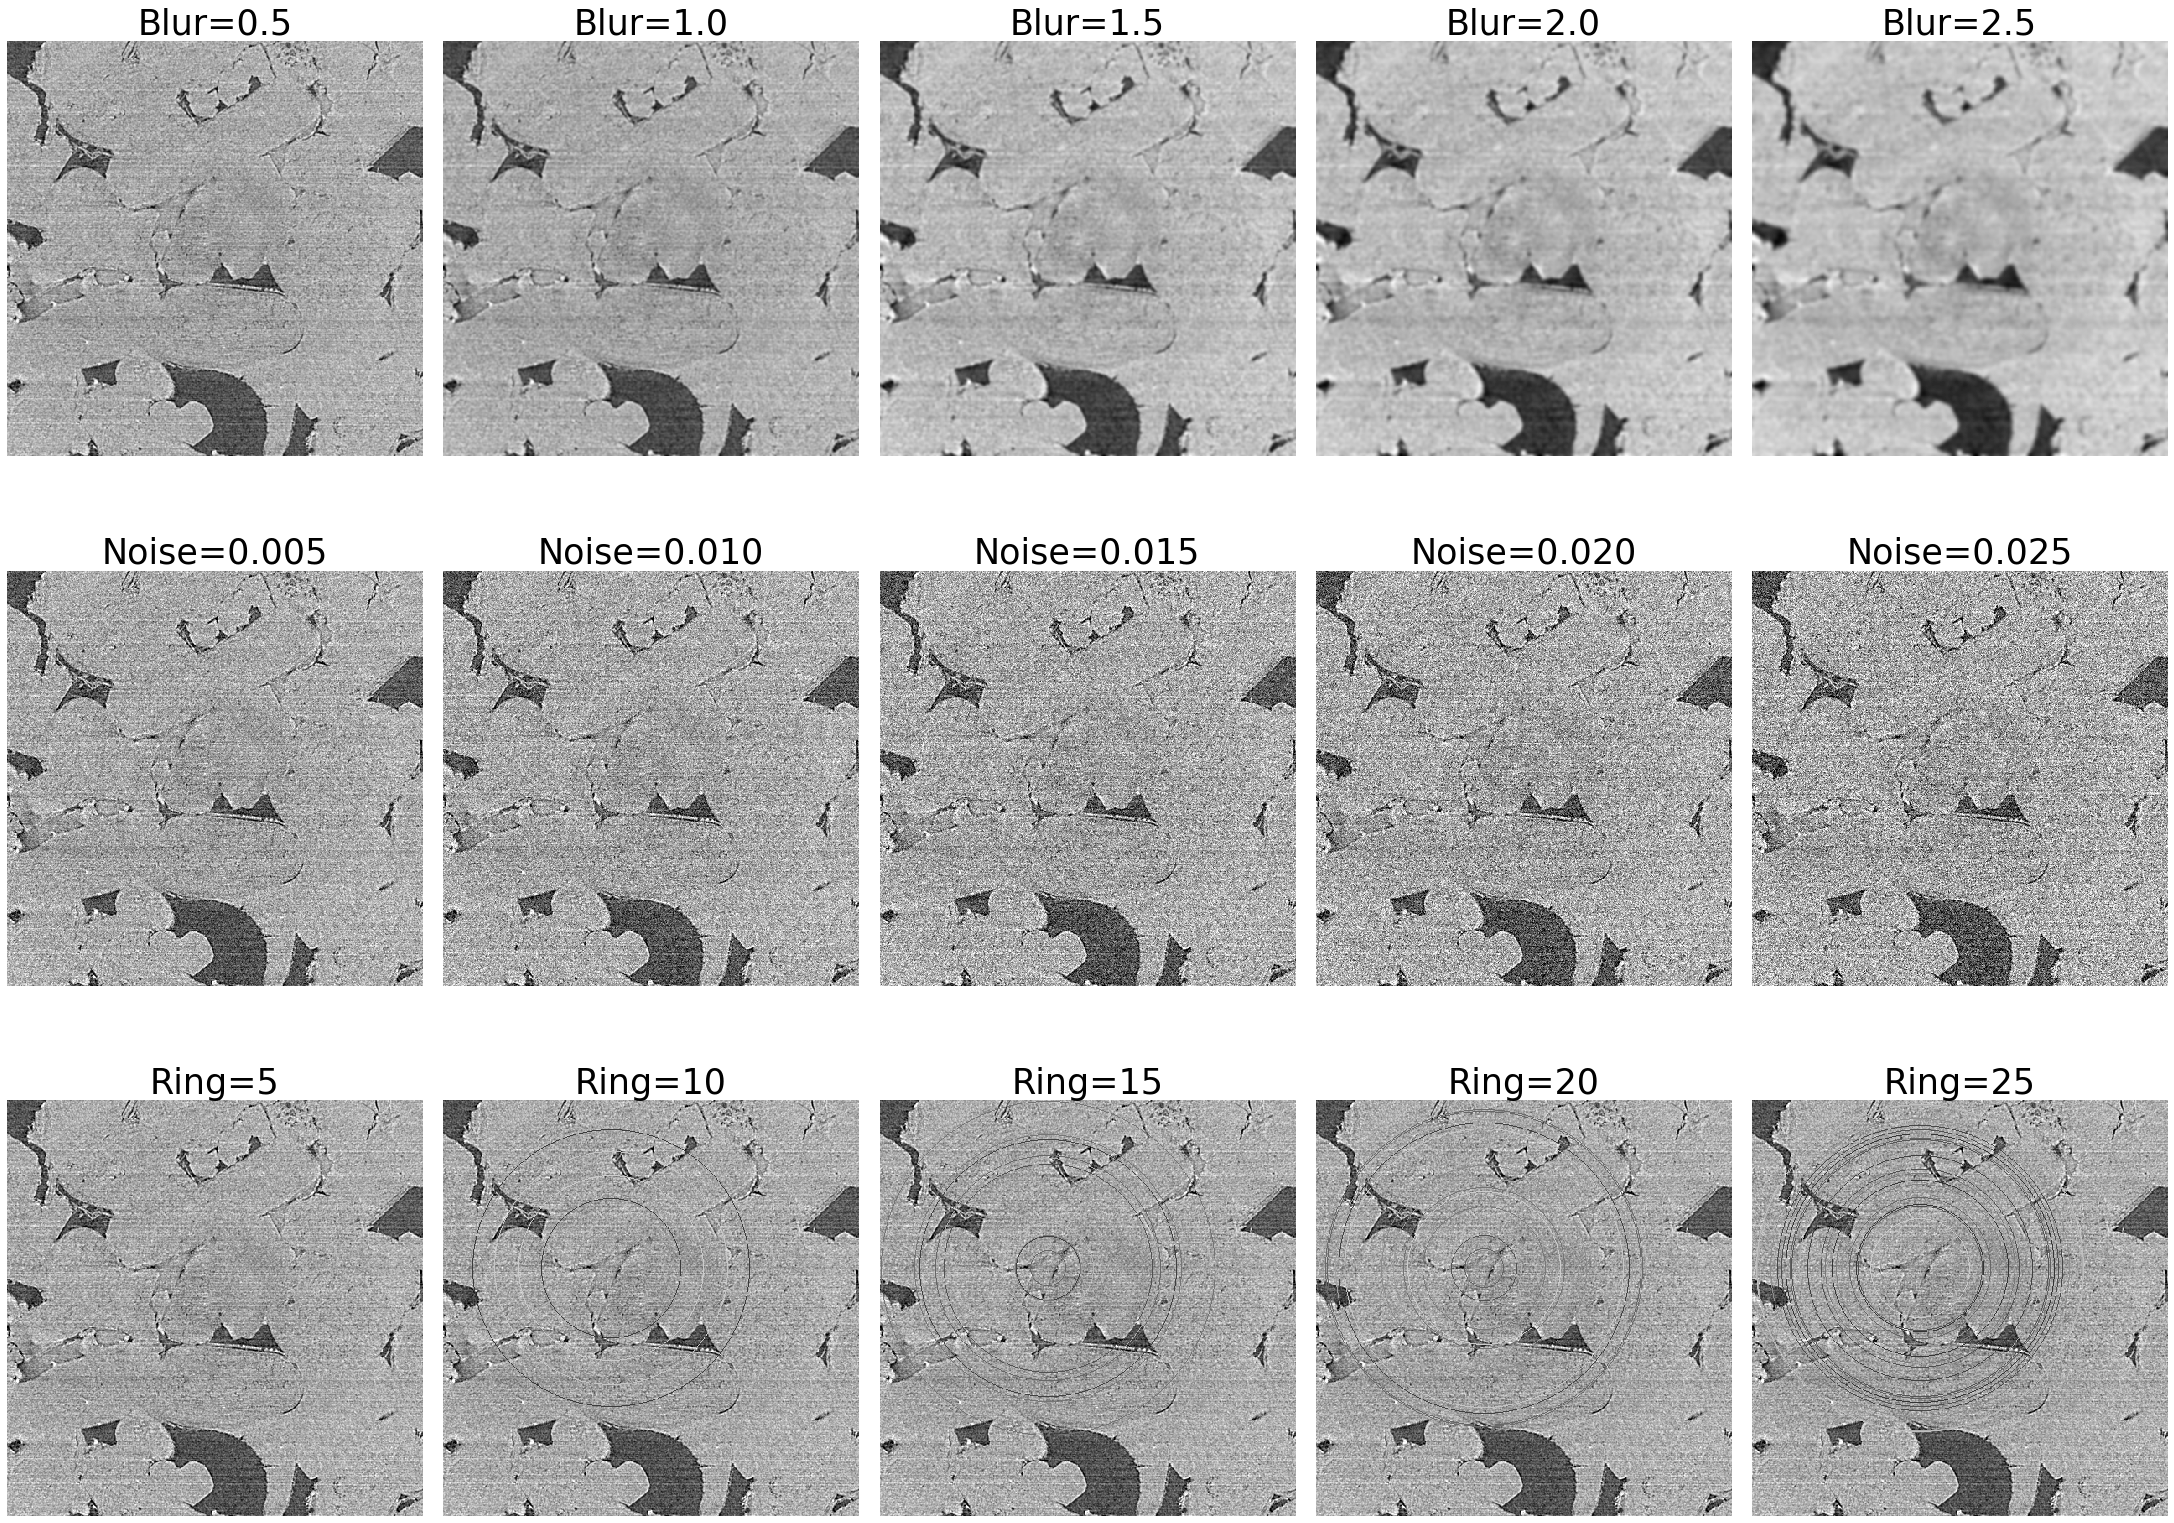
\includegraphics[width=1\textwidth]{\dir/figs/noisetest2}
  \caption{}
  \label{noisetest}
\end{figure}

The CNN segmentation was tested on this image degradation series and the segmentation results are shown below in Fig.\ref{noisetestseg}, and major misclassifications were marked in red circle in Fig.\ref{segmisclassification}.  

For the blurred series (the first row), except a minor degree of blurring (blur=0.5), the CNN model produce sub-standard segmentation that many of the pore space and fluids were misclassified. The segmentation even misclassified very distinguishable oil as rock, this is because the training set has none of such blurring so the model is very sensitive to blurring. To reduce the sensitivity for future data sets in the future training, blurred data set by different methods (e.g. mean/median filter, Gaussian blur etc.) can be trained with.

For the noised series (the second row), all segmentation images are sub-standard, this shows an even worse resistance of the CNN model to Gaussian noise. The pattern of misclassification in this series is very different to the blurred series. The model misclassify the majority of oil as brine, and the rock segmentation was also heavily noised. This result is surprising because the training set itself has various degree of noise, the possible explanation is that the CNN model is trained on a different kind of noise than Gaussian noise. To increase the model resistance to various kind of noise, the model should be future trained with different kind of artificial noise. 

The ring artefact series (the third row) shows relatively good segmentation result that only the last segmentation result has obvious major misclassification. This is also surprising because the training set does not suffer from serious ring artefact. However the model shows good resistance to low to intermediate artificial ring artefact.

\begin{figure}[htbp]
  \centering
  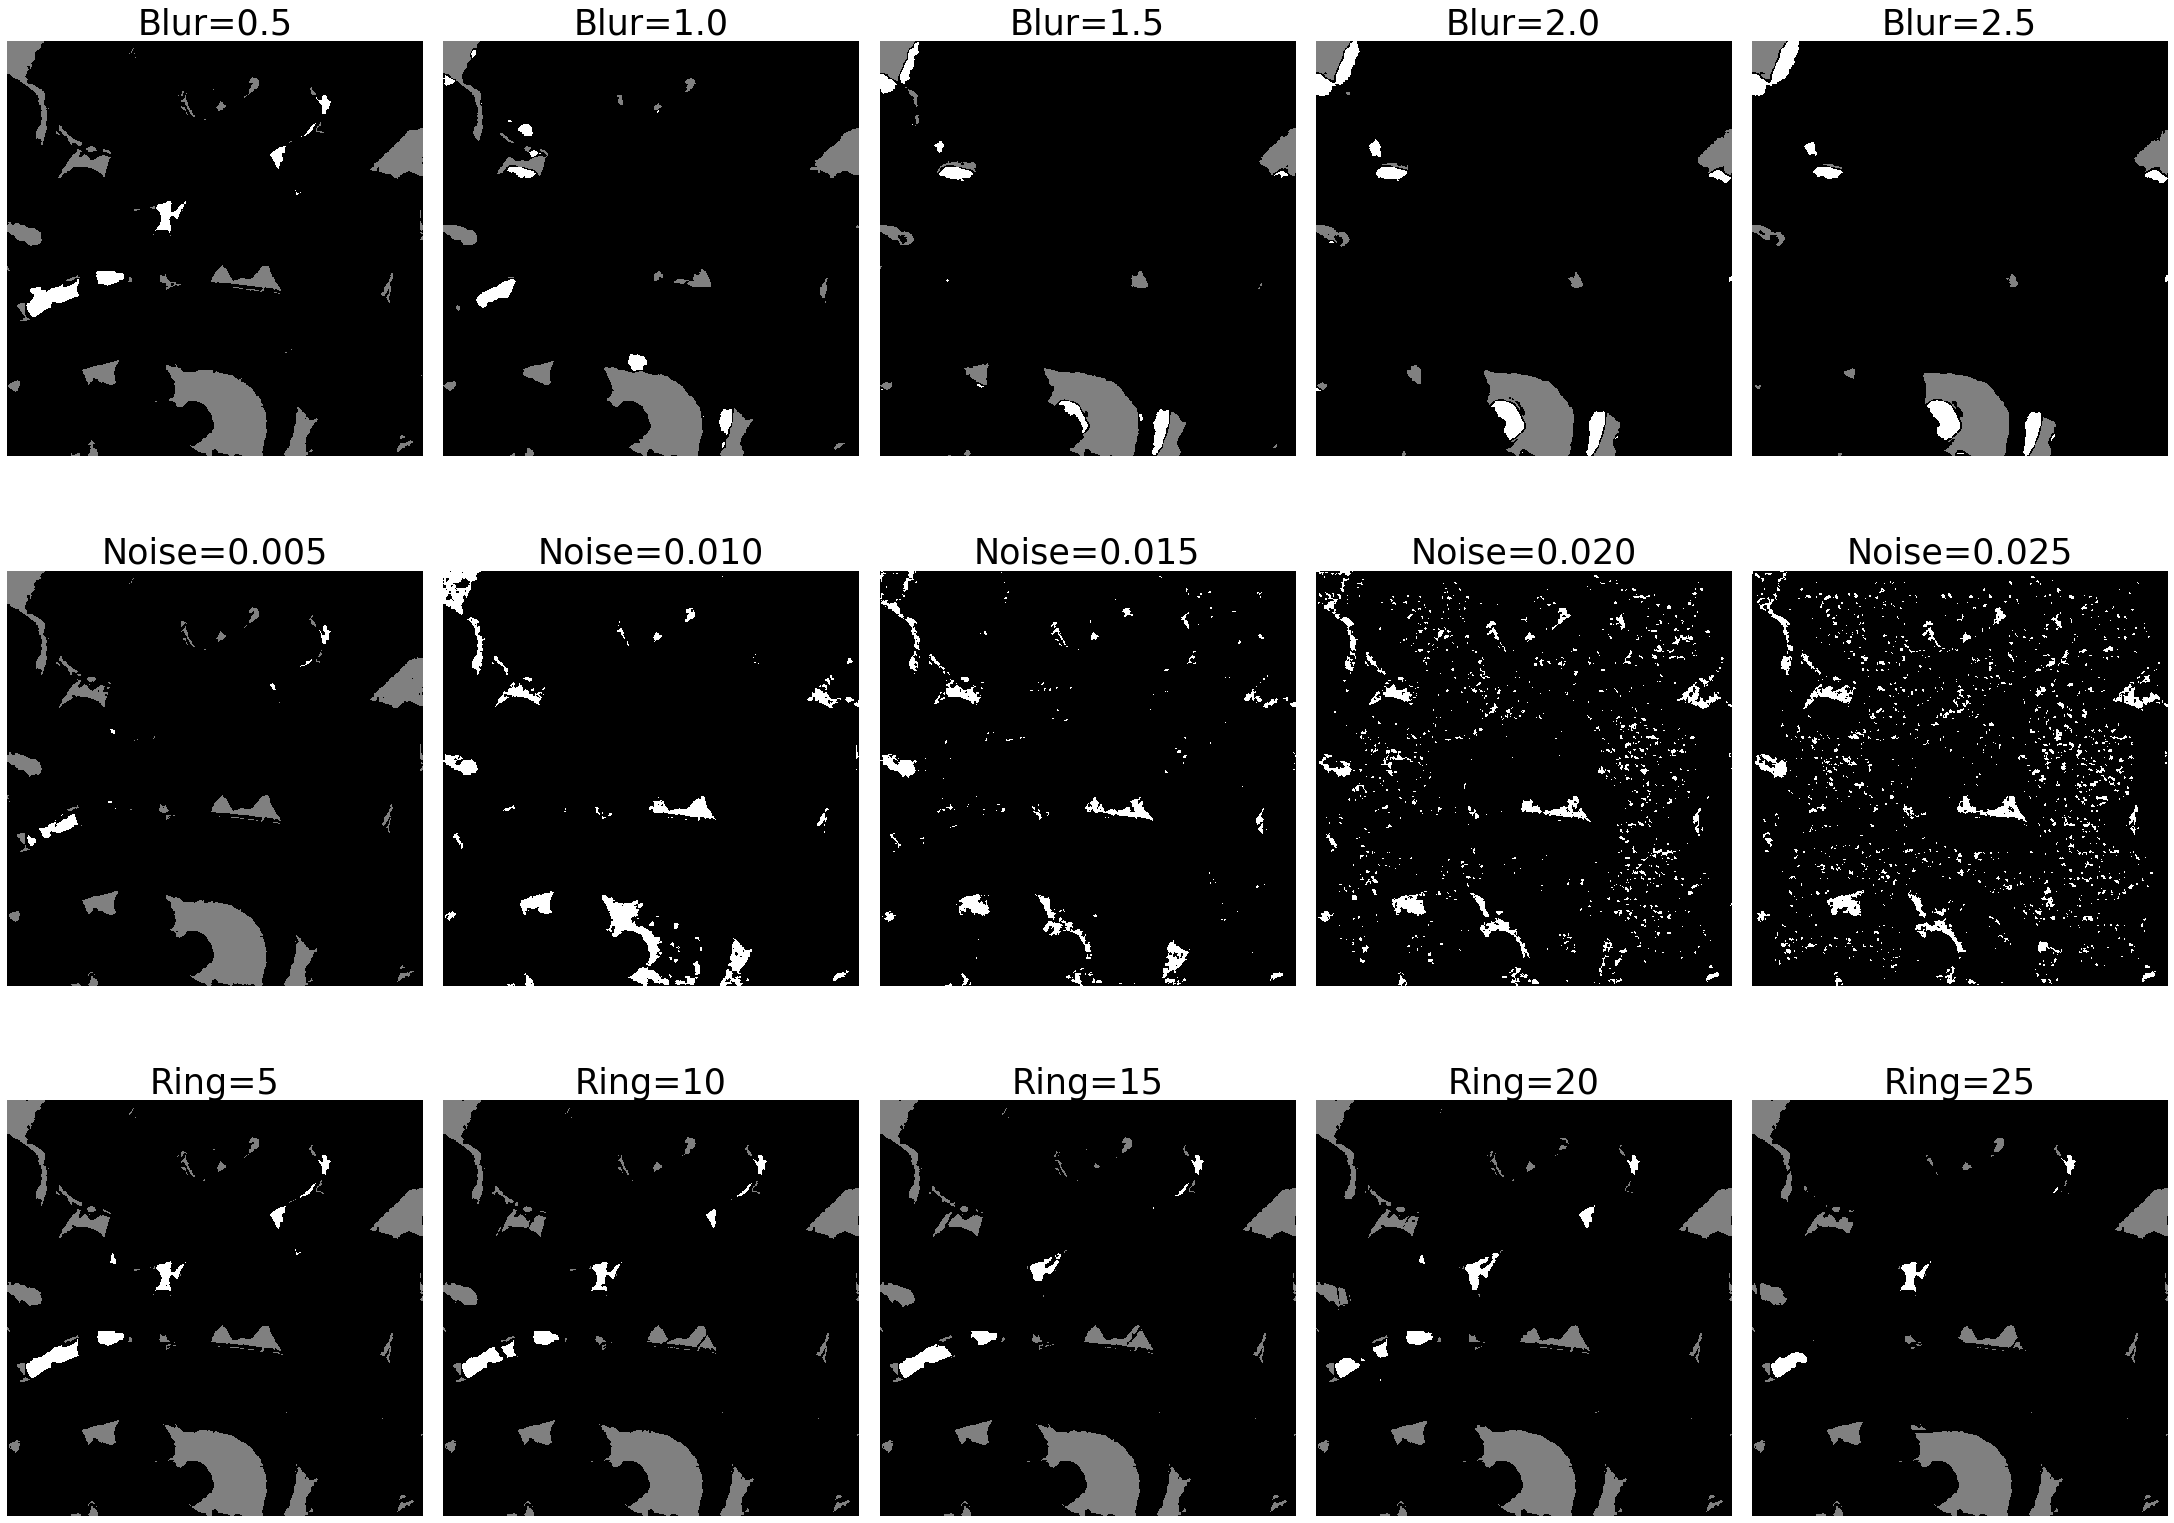
\includegraphics[width=1\textwidth]{\dir/figs/noisetest2seg}
  \caption{}
  \label{noisetestseg}
\end{figure}

\begin{figure}[htbp]
  \centering
  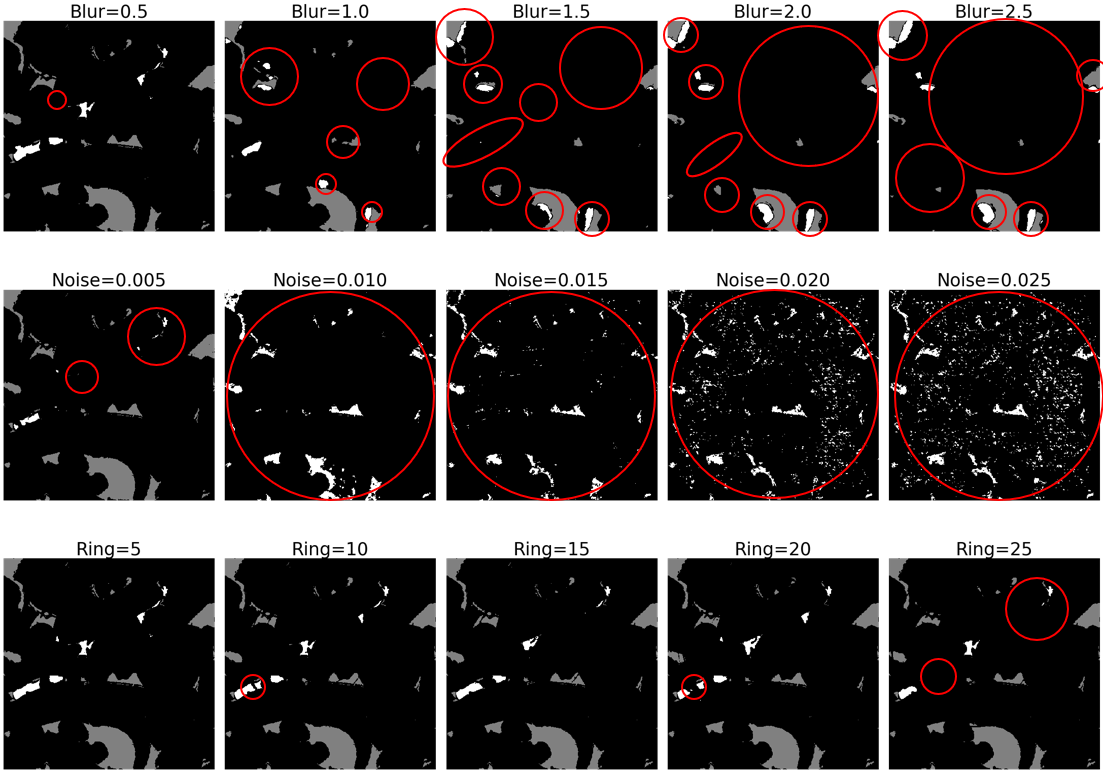
\includegraphics[width=1\textwidth]{\dir/figs/segmisclassification}
  \caption{}
  \label{segmisclassification}
\end{figure}

The three-phase mean accuracy and IoU of these three degraded series are plotted in Fig.\ref{robustness}. The trend of degradation resistance is showing clearly that for the first set of Gaussian blurred image, the segmentation quality starts to decrease at the second degradation step, and gradually stabilised in further steps. The noised series of Gaussian noised image suffered from the most severe plunge in segmentation quality, and it does not show any sign of stabilisation within the tested degradation steps. The third kind of degradation - the ring artefacts almost did no harm to the segmentation quality. 

\begin{figure}[htbp]
  \centering
  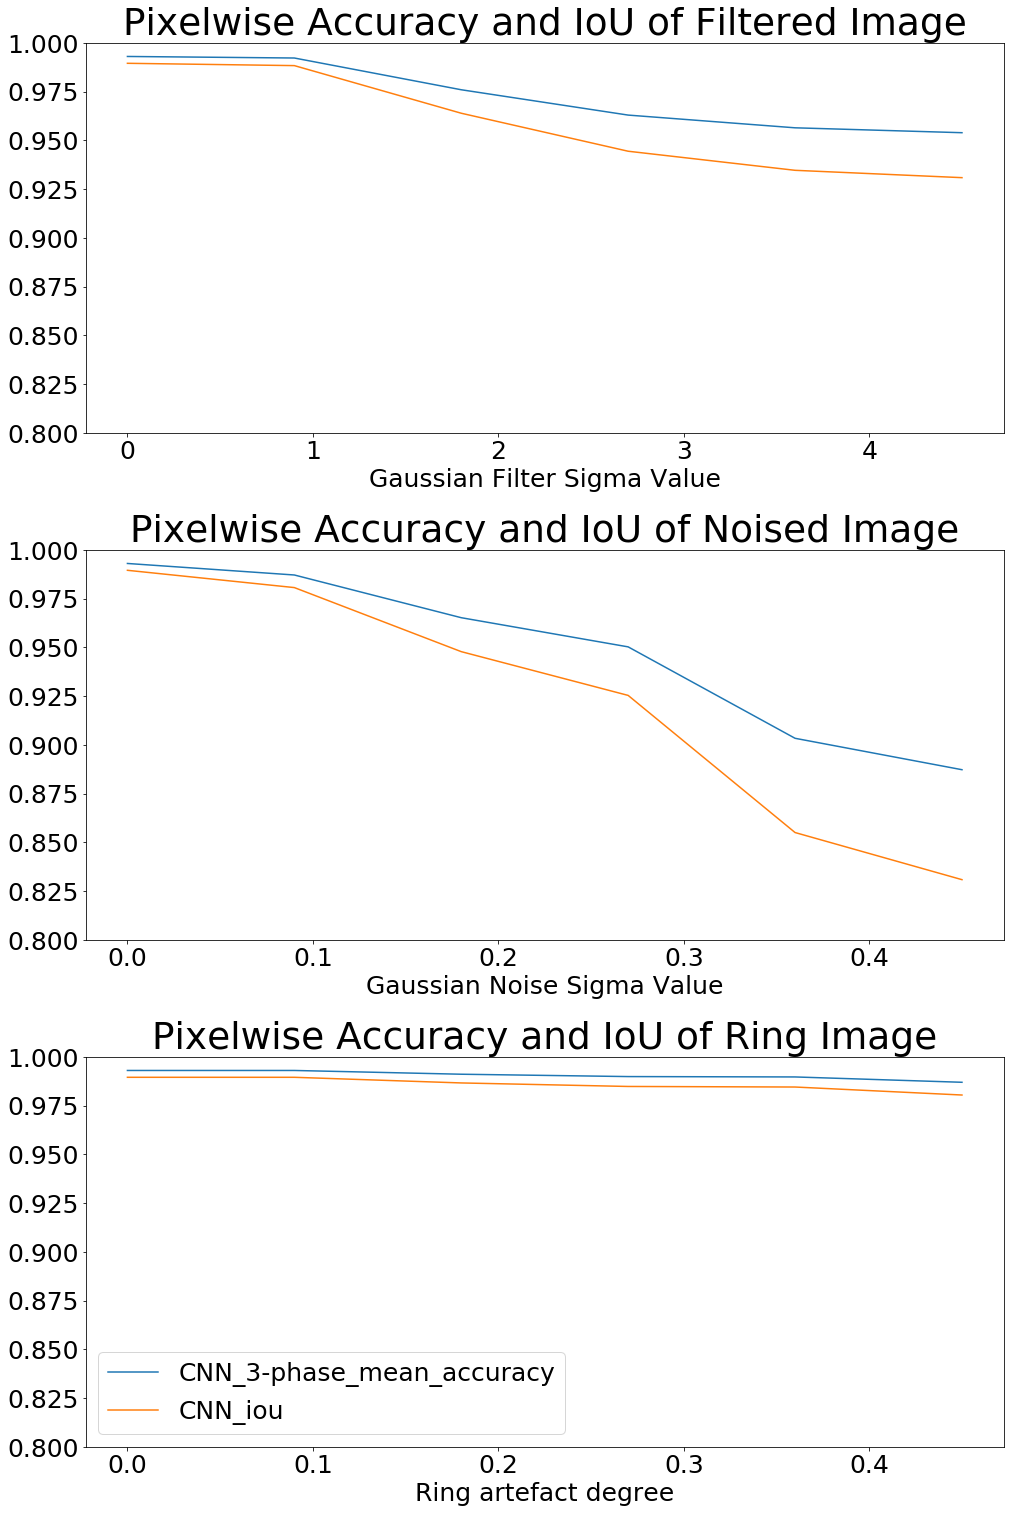
\includegraphics[width=1\textwidth]{\dir/figs/robustness}
  \caption{}
  \label{robustness}
\end{figure}

The above experiments shows that the trained CNN model has different robustness on scaling blurring, noising and ring artefact. The model can resist a minor degree of Gaussian blurring, for more severe blurring, the segmentation quality decreased and gradually stabilised. Compared with blurring, the model has lower resistance to Gaussian noise, and the segmentation quality will decrease without stabilisation with scaling Gaussian noise. For artificial ring artefacts, the CNN model has strong resistance and the segmentation result is very robust and only minor misclassification is caused.

This result is surprising because from human eye perspective, the blurring and noising cause less impact on the recognition of the object than ring artefacts. However from machine's perspective, the artificial ring artefact cause the least obstruction on segmenting artificial ring artefact affected images. This shows a completely different way of vision between human and machine. This observation has also been made by various of other researches like \citet{nguyen2015deep,su2019one,goodfellow2014explaining}. They suggested that although the image only changed a little in human's perspective, it changed drastically in computer vision. 

For example \citet{goodfellow2014explaining} reported that, by adding a carefully crafted systematic noise to a panda image, the trained deep learning neural network would recognise the panda as a gibbon with 99.3\% confidence, although the image appears still a panda in human eyes (Fig.\ref{goodfellow}). This means that the state-of-art deep learning neural networks can be easily 'fooled' by crafted noise without noticing by human eyes.

\begin{figure}[htbp]
  \centering
  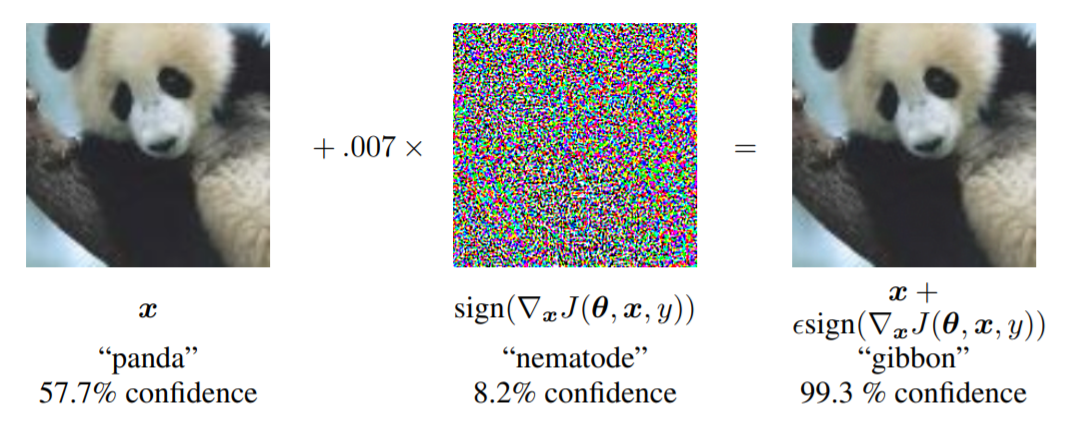
\includegraphics[width=1\textwidth]{\dir/figs/goodfellow}
  \caption{}
  \label{goodfellow}
\end{figure}

\citet{su2019one} reported that, even with one-pixel that carefully changed on the input image, the deep neural network image classification model can make totally different prediction (Fig.\ref{su}). The input images were altered by one pixel using a specific method, and caused very disrupted classification result.

\begin{figure}[htbp]
  \centering
  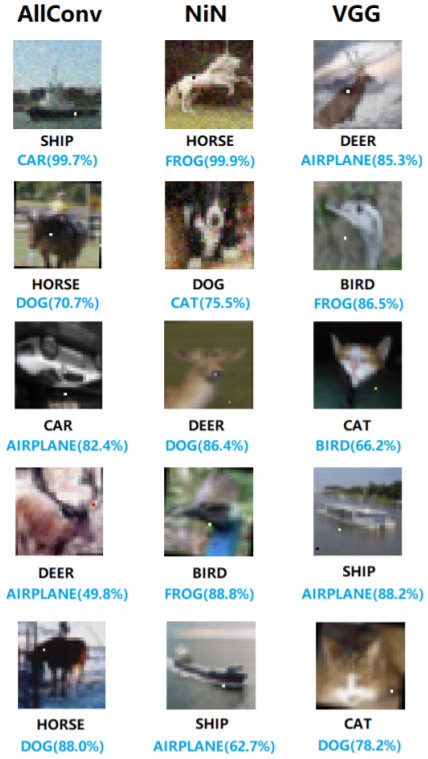
\includegraphics[width=0.5\textwidth]{\dir/figs/su}
  \caption{}
  \label{su}
\end{figure}

The other way around, images that make zero sense to human eyes, if the pattern is carefully generated, can be recognised as familiar objects by the machine with high confidence. \citet{nguyen2015deep} reported examples of such images (Fig.\ref{imagenet}). 

\begin{figure}[htbp]
  \centering
  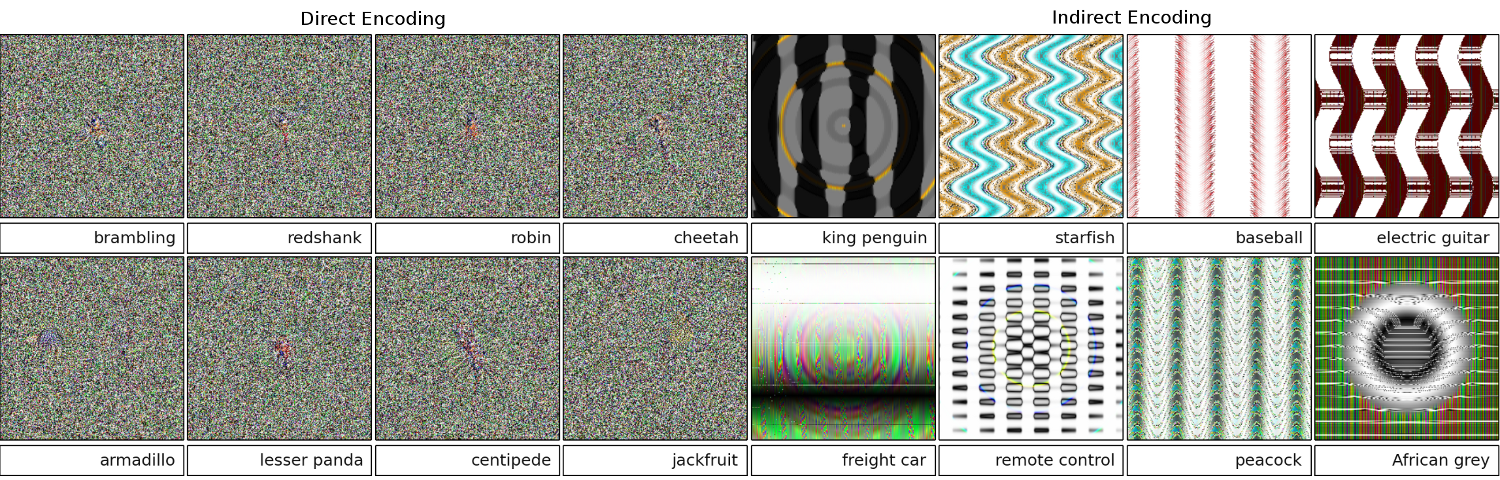
\includegraphics[width=1\textwidth]{\dir/figs/imagenet_16_images_horizontal_0}
  \caption{}
  \label{imagenet}
\end{figure}

These studies helps with the understanding of why the artificial blurring and noising can dramatically affect the segmentation result. The global, systematic alteration to the input image has much more impact on machine's judgement than the alteration appears to human eyes. Unlike the blurring and noising which is global, the artificial ring artefact is relatively local and does not affect the entire image, so the CNN can perform much better resistance to such degradation. This highlights the very complicated sensitivity of computer vision by deep neural networks that we must pay attention to, this also implies that in future training, data sets with various of image alteration should be included to increase the robustness of the CNN model.

\section{Conclusion}
The CNN segmentation can significantly improve the segmentation workflow for multiphase flow \textmu CT images. The advantages are five-fold. Firstly once a network for segmenting multiphase flow images is trained, it can be applied to future data without re-train. Second, once a network is trained it can function without a high quality reference image at time zero, allowing segmentation of any data set that lacks such a reference. Thirdly the segmentation is the direct output from reconstruction image, and so the considerable time consumed by pre-processing (tuning of filtering, registration, masking etc.) is no longer required. This is significant because for fast synchrotron \textmu CT data set, the data processing time is considerably long compared with time used for interpretation. Fourthly, the algorithm is capable for highly noised images, which is extremely limiting for conventional processing paths. Finally, the performance of the CNN network improves as more data it has seen, it evolves itself when it is used. Overall the CNN segmentation is a powerful and efficient tool for \textmu CT image segmentation, especially for extra-large and noisy data set.

